% !TeX program = pdflatex
% Compilation depuis la racine : latexmk slides_presentation.tex
\documentclass[11pt,aspectratio=169]{beamer}

\usepackage[utf8]{inputenc}
\usepackage[T1]{fontenc}
\usepackage[french]{babel}
\usepackage{lmodern}
\usepackage{microtype}
\usepackage{graphicx}
% Conserver les polices incorporées à la page de garde PDF, sans substitution.
\pdfinclusioncopyfonts=1
\graphicspath{{images/}}

% Le thème est isolé pour pouvoir être personnalisé indépendamment du contenu.
\usepackage{beamertheme/beamerthemeMermozSaclay}

\title[Présentation ENS \& FAQ prépa]{Présentation ENS\\\& FAQ prépa}
\subtitle{Visio}
\author{Lubin Bénéteau} % Ajouter le nom de l'intervenant ici.
\institute{Lycée Jean Mermoz \quad\textbullet\quad ENS Paris-Saclay}
\date{6 novembre 2026 à 18\,h}
\titlegraphic{%
  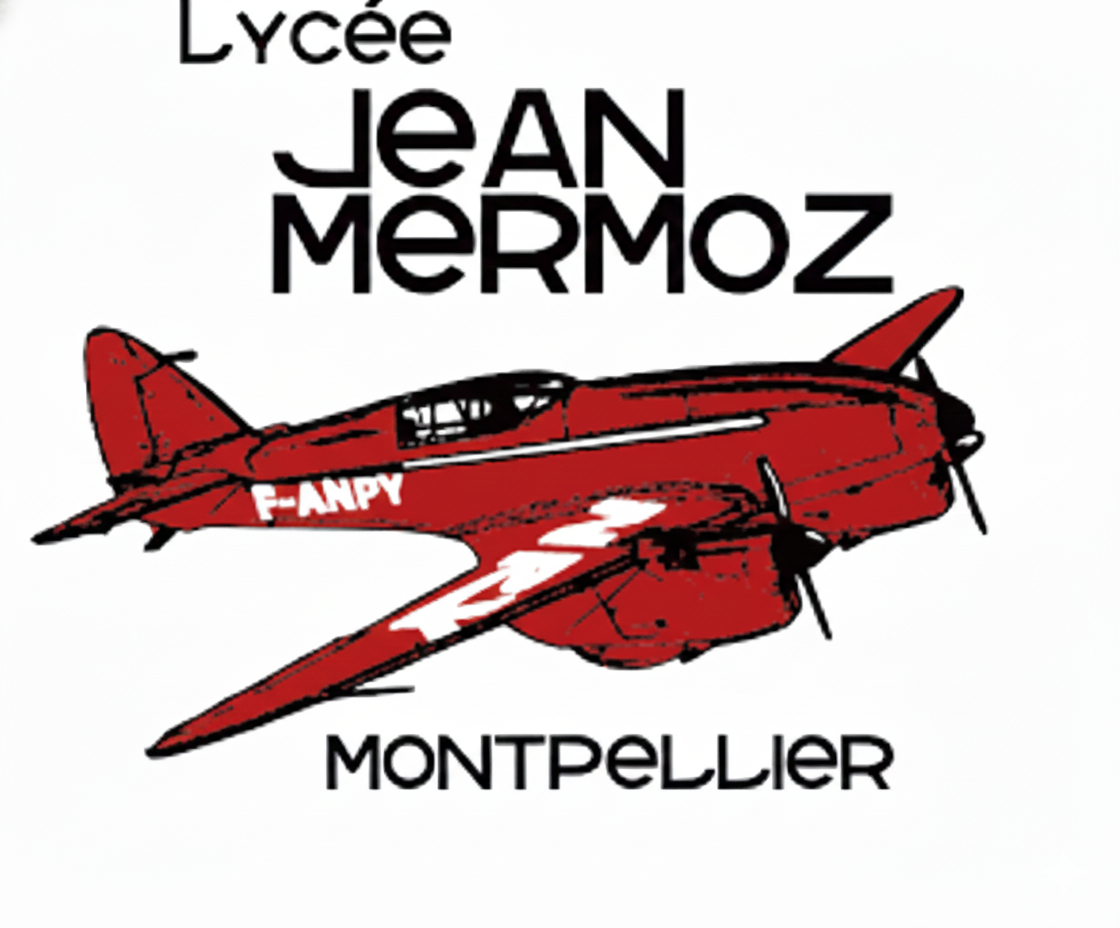
\includegraphics[height=15mm]{logo_mermoz(1).png}%
  \hspace{12mm}%
  
\includegraphics[width=51mm]{logo_ens_ups(1).png}%
}

\begin{document}

% Le PDF de référence conserve exactement la page de garde existante.
% Les métadonnées ci-dessus restent disponibles pour une future réédition.
{
\usebackgroundtemplate{%
  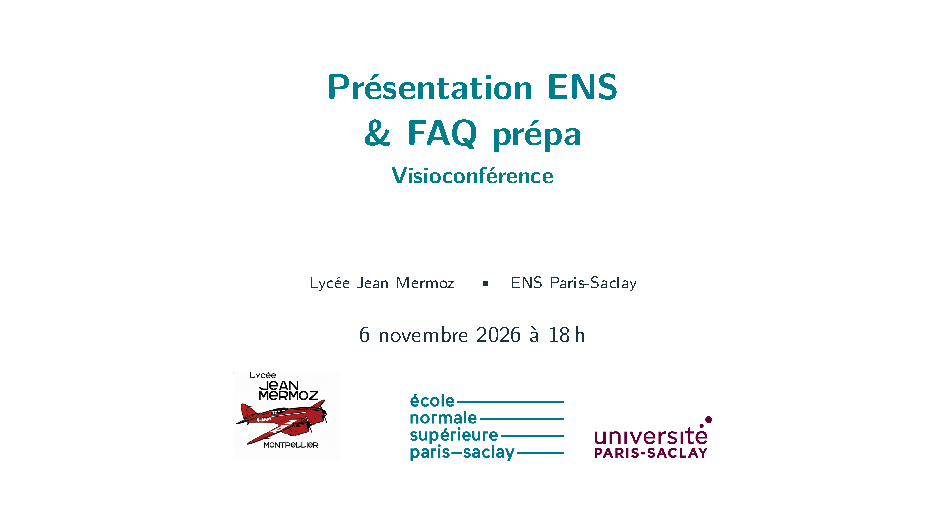
\includegraphics[width=\paperwidth,height=\paperheight]{page_de_garde.pdf}%
}
\begin{frame}[plain]
  \centering
  \vfill
  {\small Lubin Bénéteau}
  \vfill
\end{frame}
}

\begin{frame}{Sommaire}
  \begin{enumerate}
    \setlength{\itemsep}{5mm}
    \item Présentation des anciens
    \item L'ENS : associations et sports
    \item Les doubles diplômes de l'ENS
    \item Les grandes questions sur la prépa
    \item FAQ
    \item Lorem ispum
  \end{enumerate}
\end{frame}

\section{Présentation des anciens}
\begin{frame}{Présentation des anciens}
  \begin{columns}[T,onlytextwidth]
    \begin{column}{\textwidth}
      \textbf{Tour de table}\par\medskip
      \begin{itemize}
        \setlength{\itemsep}{3mm}
        \item Promo Mermoz et date d'entrée à l'ENS
        \item 1A : L3, majeure et mineure
        \item 2A : quel M1 ?
        \item 3A : M2R, ASP (DD, ARPE), césure\ldots
        \item 4A : ASP (DD, ARPE)\ldots
        \item Ce que l'on veut faire plus tard ? 
      \end{itemize}
    \end{column}
  \end{columns}
\end{frame}

\section{L'ENS : associations et sports}
% Sources institutionnelles détaillées dans SOURCES.md (diapositive 4).
\begin{frame}{L'ENS : associations et sports}
  \begin{columns}[T,onlytextwidth]
    \begin{column}{0.48\textwidth}
      {\large\color{DauphineBleu}\bfseries La vie associative}\par\medskip
      \begin{itemize}
        \setlength{\itemsep}{4mm}
        \item \textbf{BDE et Kfet} : soirées étudiantes + ``foyer''.
        \item \textbf{Arts et culture} : BDA, éloquence, conférence, musique, fanfarre, théâtre, cinéma\ldots
        \item \textbf{S'engager} : solidarité avec la SoNo, écologie avec Terre à Terre.
      \end{itemize}
    \end{column}
    \begin{column}{0.47\textwidth}
      {\large\color{DauphineBleu}\bfseries Le sport sur le campus}\par\medskip
      \begin{itemize}
        \setlength{\itemsep}{4mm}
        \item \textbf{Pratiquer} : foot, hand, volley, rugby, course, escalade, danse, rock, raquettes\ldots
        \item \textbf{Compétition} : Matchs contre les autres écoles du plateau / de Paris 
        \item \textbf{Se retrouver} : InterENS, ENSympiades et tournois avec le BDS.
      \end{itemize}
    \end{column}
  \end{columns}
  \vfill
  {\color{DauphineBleu}}
\end{frame}

\section{Les doubles diplômes de l'ENS}
% Exemples confirmés par la page officielle du parcours Interface, voir SOURCES.md.
\begin{frame}{Les doubles diplômes de l'ENS}
  Compléter sa formation dans un établissement partenaire,\par
  dans le cadre d'un \textbf{double diplôme}.
  \vspace{6mm}
  \begin{description}[Ingénierie et statistiques]
    \setlength{\itemsep}{4mm}
    \item[Ingénierie et statistiques] ENSAE Paris, École des Ponts, Mines Paris
    \item[Affaires publiques] Sciences Po, Prépa INSP
    \item[Management] HEC, ESCP, ESSEC
  \end{description}
  \vspace{6mm}
  \textbf{Des voies sélectives, avec un nombre de places limité.}\par
  \medskip
  \small
  Débouchée après l'ENSAE : corps des INSED (haute fonction publique, comme parès INSP (ex ÉNA)).
\end{frame}

\section{Les grandes questions sur la prépa}
\begin{frame}{Les grandes questions sur la prépa}
  \begin{enumerate}
    \setlength{\itemsep}{4mm}
    \item \textbf{Comment se préparer au concours ?}\par
          Ça dépend cb de tps avant, physiquement/mentalement, quelle matière, etc ?
    \item \textbf{Quelle méthode de travail au quotidien ?}\par
          Ça dépend de la matière, des envies, capacité de travail, etc 
    \item \textbf{Comment éviter de perdre ses moyens devant un sujet ?}\par
          L'avoir déjà vu sûrement...
    \item \textbf{les khôlles, quelles méthodes ?}\par
          Ça dépend de la khôlle, ça dépend de la note visée/objectif
  \end{enumerate}
\end{frame}

\section{FAQ}
\begin{frame}{FAQ}
  {\Large\color{DauphineBleu}\bfseries À vous les amis}\par
  \medskip
  Posez vos questions à l'oral ou dans le chat.
\end{frame}

\begin{frame}{last frame}
  \centering
  {\LARGE\color{DauphineBleu}\bfseries Merci ! Ciao}\par
  \vspace{8mm}
  {\large }\par
  \medskip
  {\large }\par
  \vspace{10mm}
  Les anciens de Mermoz
\end{frame}

\end{document}
